% all the content of the poster goes here.
% uses greenboxes, blueboxes, redboxes as shown below.

\begin{greenbox}{Some info on lengths}
  \begin{center}
    \begin{tabular}[]{l c}
      \toprule
      \multicolumn{2}{c}{Lengths, width and margins}\\
      \midrule
      hoffset & \the\hoffset\\
      voffset & \the\voffset\\
      parskip & \the\parskip\\
      parindent & \the\parindent\\
      leftmargin &  \the\leftmargin\\
      rightmargin & \the\rightmargin\\
      topmargin & \the\topmargin\\
      oddsidemargin & \the\oddsidemargin\\
      evensidemargin & \the\evensidemargin\\
      textwidth & \the\textwidth\\
      textheight & \the\textheight\\
      paperwidth & \the\paperwidth\\
      paperheight & \the\paperheight\\
      headheight & \the\headheight\\
      footskip & \the\footskip\\
      %footheight= \the\footheight\\
      \bottomrule
    \end{tabular}
  \end{center}
\end{greenbox}

%-----------------------------------------------------------------------
\begin{greenbox}{Abstract}
  \blindtext
\end{greenbox}
%-----------------------------------------------------------------------


%-----------------------------------------------------------------------
\begin{greenbox}{A first box}
  In the first box, there shall be some
  \[ \mathrm{F}_{\mathrm{or}}^{\mathrm{mul}} = as \]
  and furthermore,
  \begin{align*}
    some &= fancy\\
    1 &\equiv 1
  \end{align*}
  environment shall be used.
\end{greenbox}
%-----------------------------------------------------------------------

%-----------------------------------------------------------------------
\begin{greenbox}{The second box}
  \begin{itemize}
  \item First
  \item Second
  \item Third and forth
  \end{itemize}
\end{greenbox}
%-----------------------------------------------------------------------

%-----------------------------------------------------------------------
\begin{greenbox}{Graphics work, too!}
  Some beautiful plot is this one:\\ % short lines benefit from manual line breaks
  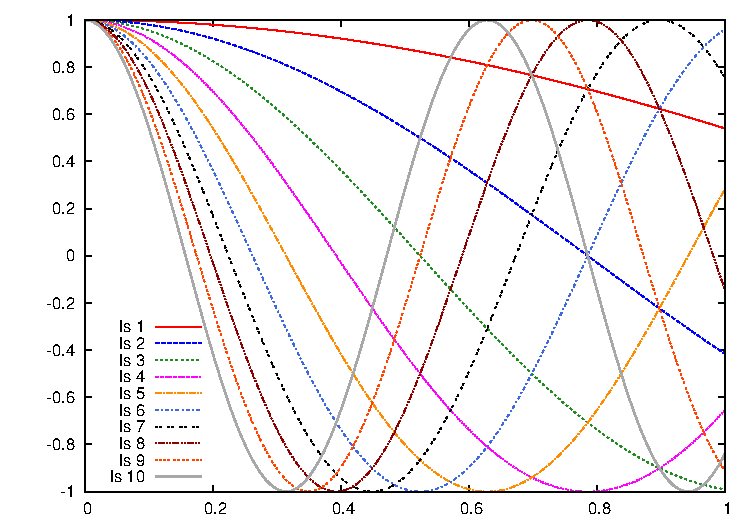
\includegraphics[width=0.9\textwidth]{images/colortest}\\
  It shows many Gnuplot linestyles with plenty of
  \begin{enumerate}
  \item thickness
  \item contrast
  \item beauty
  \end{enumerate}

\end{greenbox}
%-----------------------------------------------------------------------

\columnbreak

%-----------------------------------------------------------------------
\begin{greenbox}{Some formulas}
  A nice formula is\\
  \begin{align*}
    -1 = \mathrm{e}^{-\mathrm{i}\pi}\, .
  \end{align*}
\end{greenbox}
%-----------------------------------------------------------------------

%-----------------------------------------------------------------------
\begin{greenbox}{Blocks}

  Blocks do work, too:\\
  \begin{greenblock}{Block title}{0.95\textwidth} % hier ein grüner block
    Block content. Block formula:\\
    \[ a^2+b^2=c^2\]
  \end{greenblock}

  Also, there is text below blocks.

  \begin{minipage}{\textwidth}
    
    \begin{minipage}{0.475\textwidth}
      \begin{blueblock}{Blocks next to each other}{0.9\textwidth}
        In blue, this time.
      \end{blueblock}
    \end{minipage}
    \begin{minipage}{0.475\textwidth}
      \begin{redblock}{Important block}{0.9\textwidth}
        Muy importante!
      \end{redblock}
    \end{minipage}
  \end{minipage}

\end{greenbox}

\begin{redbox}{Outlook}
  Outlook is either something you want to do next or a M\$ program.
\end{redbox}

\begin{bluebox}{Blue velvet}
  Boxes in other colors work as well.\\
  Even blue ones.
\end{bluebox}

%-----------------------------------------------------------------------
